\chapter{Experiments}
\label{chp:experiments}

The \rrtfunnel{} algorithm developed this far will now be tested in a simulation
experiment where a simple unicycle model of an airplane is set to traverse a
small strip of forest. The simulation environment can be seen in
figure~\cref{fig:simulated-forest}, where the airplane starts at one end of the
obstacle forest, and is set to traverse the strip of forest and reach any
\((x,y)\) position in a circle of radius five surrounding the endpoint thirty
five meters ahead.

\begin{figure}
  \centering
  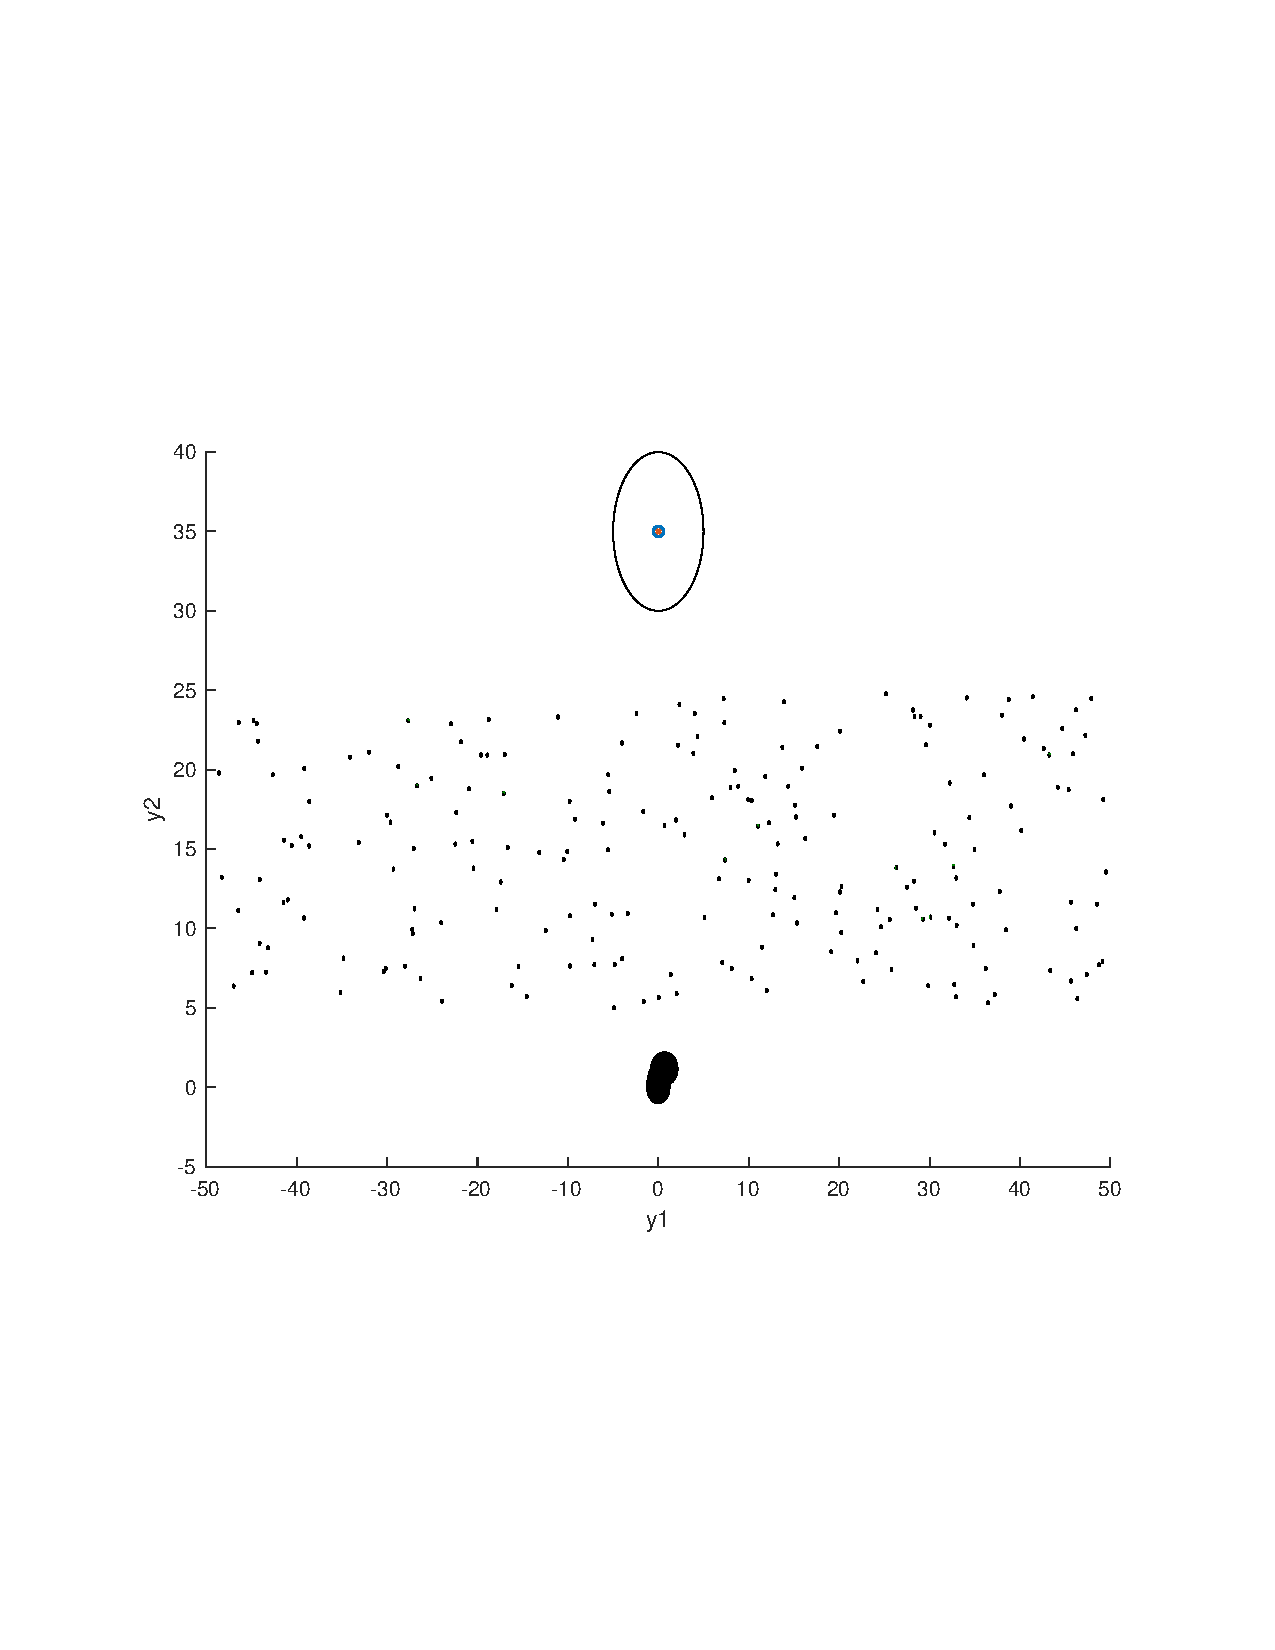
\includegraphics[width=.8\textwidth]{figures/experiments/simulated-forest} \caption{The
    experiment environment.}
  \label{fig:simulated-forest}
\end{figure}

\section{Testing the \rrtfunnel{} algorithm}

The experiment section starts out by generating a random strip of forest for
which the airplane has to navigate through in \cref{sec:Poisson-Process}. Next
it expands from the single point model in \cref{eq:model-dynamics} to
incorporate the actual size of the model in \cref{subsec:deciding-model-size},
and then shows how to expand the size of the funnels to incorporate the airplane
model in \cref{subsec:expand-funnel}. It then continues to show the initial
motion primitive set and the \ac{LQR} controller weightings in
\cref{subsec:initial-motion-primitive,subsec:lqr-cost}. In
\cref{subsec:check-vehicle-in-funnel} it employs a \textit{Monte-Carlo}
simulation in order to verify that the nonlinear system model \textit{does}
stays within the calculated funnels. Later it shows that the funnel composition
guarantees are lost due to the non-convergence in the y-direction of the funnel
space in \cref{subsec:funnel-no-composable}, until finally presenting the
results of the \rrtfunnel{} algorithm benchmarked against a conservative
\ac{RRT} motion planner which does not handle the uncertainty that is provided
by the cross-wind in \cref{sec:experiments-final}.

\subsection{Generating the obstacle forest (Poisson processes)}
\label{sec:Poisson-Process}

In order to generate the obstacle field for the experiments, which is to
resemble a forest, a \textit{spatial Poisson process} is employed. Poisson
processes are used to model random configurations of points in space, and hence
are well suited for generating a different obstacle forest for each simulation
run~\cite{Kroese_2014}. For the experiments below, a forest will be the special
case of realizing a spatial Poisson process on \(\R^2\).

A Poisson process requires a few key parameters. Firstly, \(\lambda\) is the
intensity of the spatial process, deciding the density of the generated forest,
and hence the difficulty in traversing it. For these experiments, the intensity
will be held constant for each experiment run, and not vary with points in space
\ie the process is homogeneous.

The algorithm for realizing a random Poisson measure in \cref{def:Poisson-def}
is taken from~\cite[Definition~1.1.1][34]{Kroese_2014} and looks like:

\begin{definition}{Generating a Poisson random measure}
  \label{def:Poisson-def}
  \begin{enumerate}
  \item Generate a Poisson random variable \(N \sim Poi(\mu(E))\).
  \item Draw \(X_1,X_2,\ldots,X_N \sim g\), where \(g(\vect{x}) = \lambda(\vect{x})/ \mu(E)\).
  \end{enumerate}
\end{definition}
where \(E\) is the set over which the points should be generated, and the
\textit{pdf} \(g(x_1, x_2) = \lambda(\vect{x})/\mu(E)\). Finally, \(\mu(E)\) is
defined as
\[
  \mu(E) = \int_{E} \lambda(\vect{x})\, \mathrm{d} \vect{x}.
\]

For the experiments the set \(E\) will be a square defined as
\[
  E = {[-\alpha, \alpha]}^2
\]
the density of the generated forest \(\lambda\) will be set to
\[
  \lambda = 0.1,\, 0.2,\, 0.3
\]
of which the resultant forest on a \(20 \times 20\) grid can be seen in
figure~\cref{fig:poisson009}.

\begin{figure}
  \begin{subfigure}[b]{0.5\textwidth} 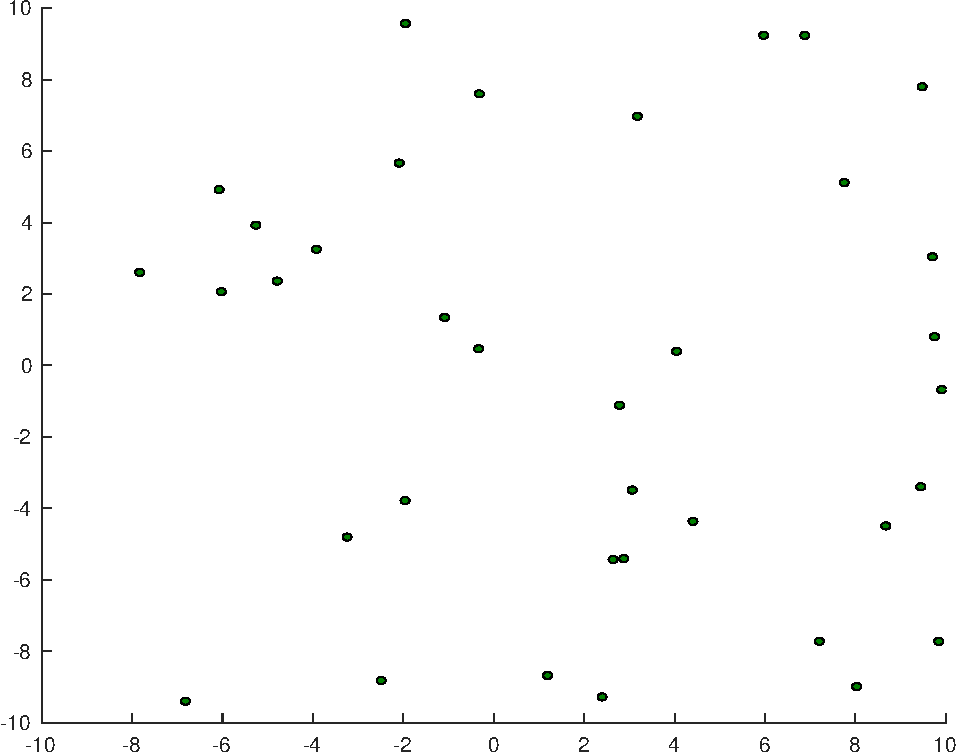
\includegraphics[width=\textwidth]{figures/experiments/poisson009}
    \caption{The resultant forest generated by a spatial Poisson process with
      intensity \(\lambda = 0.1\)}
    \label{fig:poisson009}
  \end{subfigure}%
  \;
  \begin{subfigure}[b]{0.5\textwidth}
    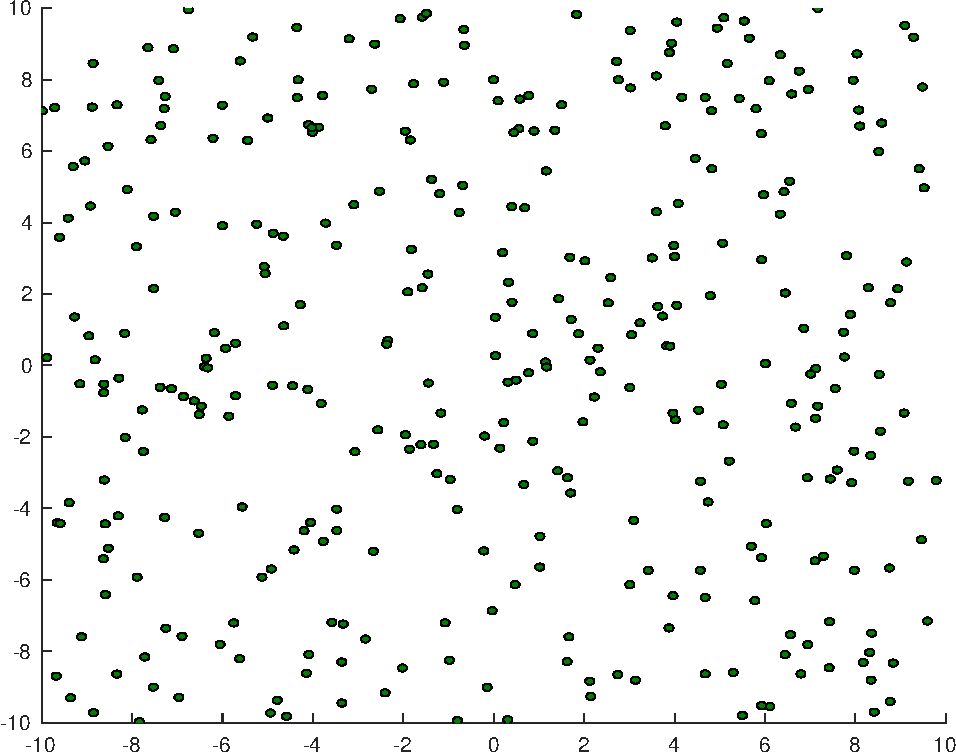
\includegraphics[width=\textwidth]{figures/experiments/poisson09}
    \caption{The resultant forest generated by a spatial Poisson process with
      intensity \(\lambda = 0.9\)}
    \label{fig:poisson09}
  \end{subfigure}
\end{figure}

\subsection{Deciding upon the size of the airplane model and the obstacles}
\label{subsec:deciding-model-size}

The funnels generated thus far are created from a point model of the airplane,
and its dynamics. If the grid that the simulations are run on are set to have an
increment of a meter, then the funnels from the basic set are given a velocity
of \([v(t)] = \si{m.s^{-1}}\), \([\theta] = \si{\radian}\), and \([\dot{\theta}]
= \si{\radian\per\second}\), where \([\cdot]\) is the unit operator. The size of
the airplane is arbitrary, and can be chosen freely, but if it is imagined as a
radio controlled aircraft, with a speed of \(10\si{m.s^{-1}}\), then a size of
\(10 \times 20 \si{\centi\metre} \) keeps everything within the realm of a
normal radio controlled aircraft and its capabilities. The mass is not relevant
for our first order dynamics, but still the airplane is assigned a mass of \(1
\si{\kilo}\), so that the translation of the model dynamics is not irrelevant. A
figure of the airplane can be seen in \cref{fig:radio-vehicle}.

\begin{figure}
  \centering
  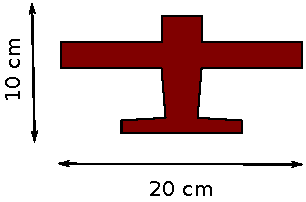
\includegraphics[width=.8\textwidth]{figures/experiments/radio-vehicle-model}
  \caption{The airplane employed in the simulation experiments.}
  \label{fig:radio-vehicle}
\end{figure}

\subsection{Expanding the size of the funnel by the size of the simulated
  airplane}
\label{subsec:expand-funnel}

The size of the airplane in the original model is a single point, and as such,
the expanded airplane model is not accounted for in the funnels. Therefore the
funnels have to be expanded in order for them to accommodate the necessary
robustness guarantees that are expected from the algorithm. However, the size of
the airplane only affects the size of the funnel ellipsis projected down into
the xy-plane. Therefore first getting the projected size of the funnel, where
\(P \colon \R^4 \rightarrow \R^2\) is a projection map with a projection matrix
\[
  P =
  \begin{bmatrix}
    I_{2 \times 2} & {0}_{2 \times 2} \\
  \end{bmatrix}
\]
such that for the projected ellipsoid
\[
  \mathcal{E}_{p} = \set{\bar{\vect{x}} \in \R^{2} \mid
    {\bar{\vect{x}}}^{T}S_{k}^{(p)}\bar{\vect{x}} \leq 1}
\]
and
\[
  S_{k}^{(p)} = {\left( PS_{k}^{-1}P^T \right)}^{-1}
\]
and \(\mathcal{E}_{p}\) is the projected set of the ellipsoid projected down
into the xy-plane as is seen in \cref{subsec:xy-cost-function}. In general an
ellipse centered at the origin is a linear transformation of the unit
circle~\cite{lay2005linear}. Exploiting this fact, expanding the radius of the
circle to encompass the airplane model. Also taking into account that the matrix
\(S_{k}\) is \textit{Positive semidefinite}, and hence can be Cholezky
factorized~\cite{lay2005linear}. The expanded ellipsis (which now contains all
the possible states of the airplane model) is:

\begin{align*}
  S_{k}^{(\mathcal{P})} &= R^{T}R \\
  \vect{x} &= R^{-1}\vect{y} \\
  \mathcal{C} &= \set{\vect{y} \in \R^2 \mid \vect{y}^{T}\vect{y} \leq 1 + r_{airplane}} \\
  \mathcal{E}_{exp} &= \set{R^{-1}\vect{y} \mid \vect{y} \in \mathcal{C}} \\
\end{align*}
where \(\mathcal{E}_{exp}\) is the ellipsoid which contains the volume of the
airplane for all verified states in the funnel, and \(r_{airplane}\) is the
widest part of the model at hand, which in this case is the wingspan. A picture
of the initial funnel and the funnel expanded around the airplane model can be
seen in figure~\cref{fig:expanded-funnel,fig:expanded-and-unexpanded}.

\begin{figure}
  \centering 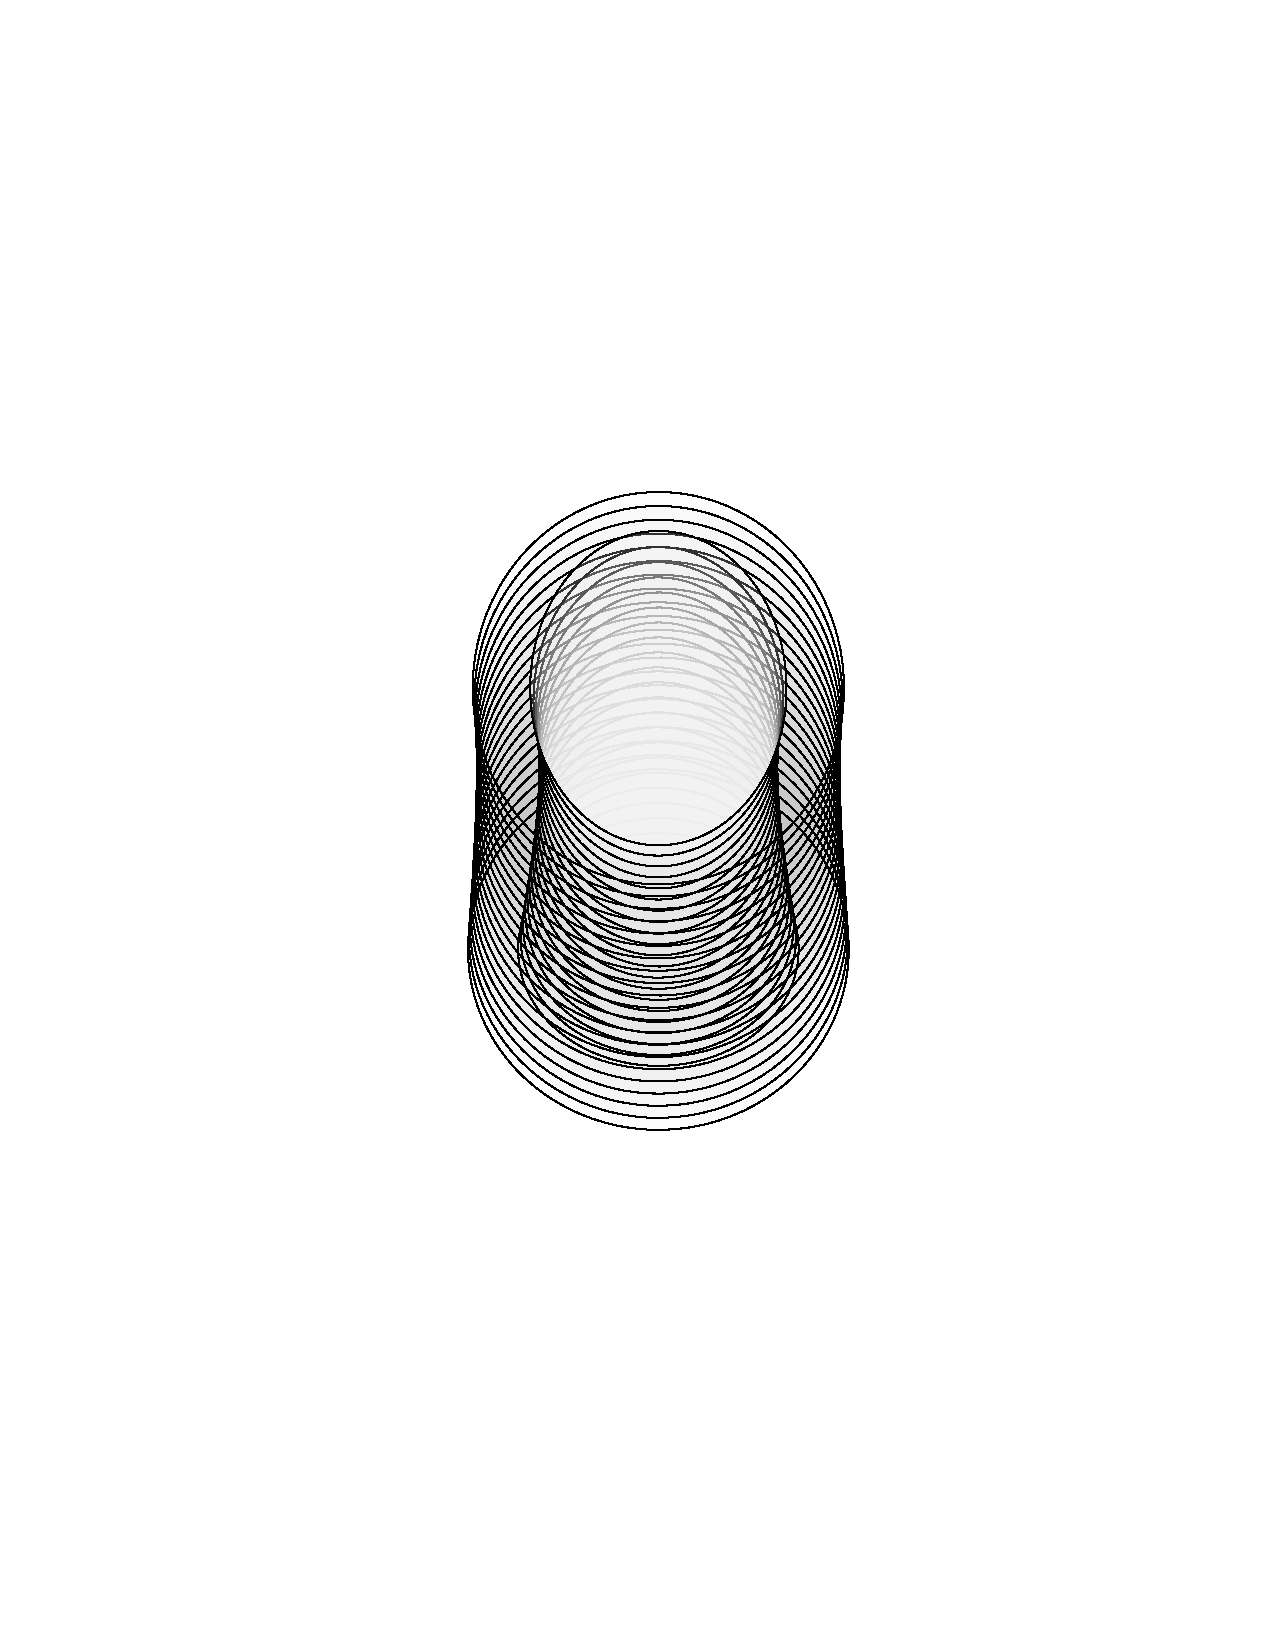
\includegraphics[scale=.7]{figures/method/expanded-funnel}
  \caption{The original funnel created from the point model, with a funnel
    expanded by a radius of 0.1 surrounding it.}
  \label{fig:expanded-funnel}
\end{figure}

\begin{figure}
  \begin{subfigure}{0.5\textwidth}
    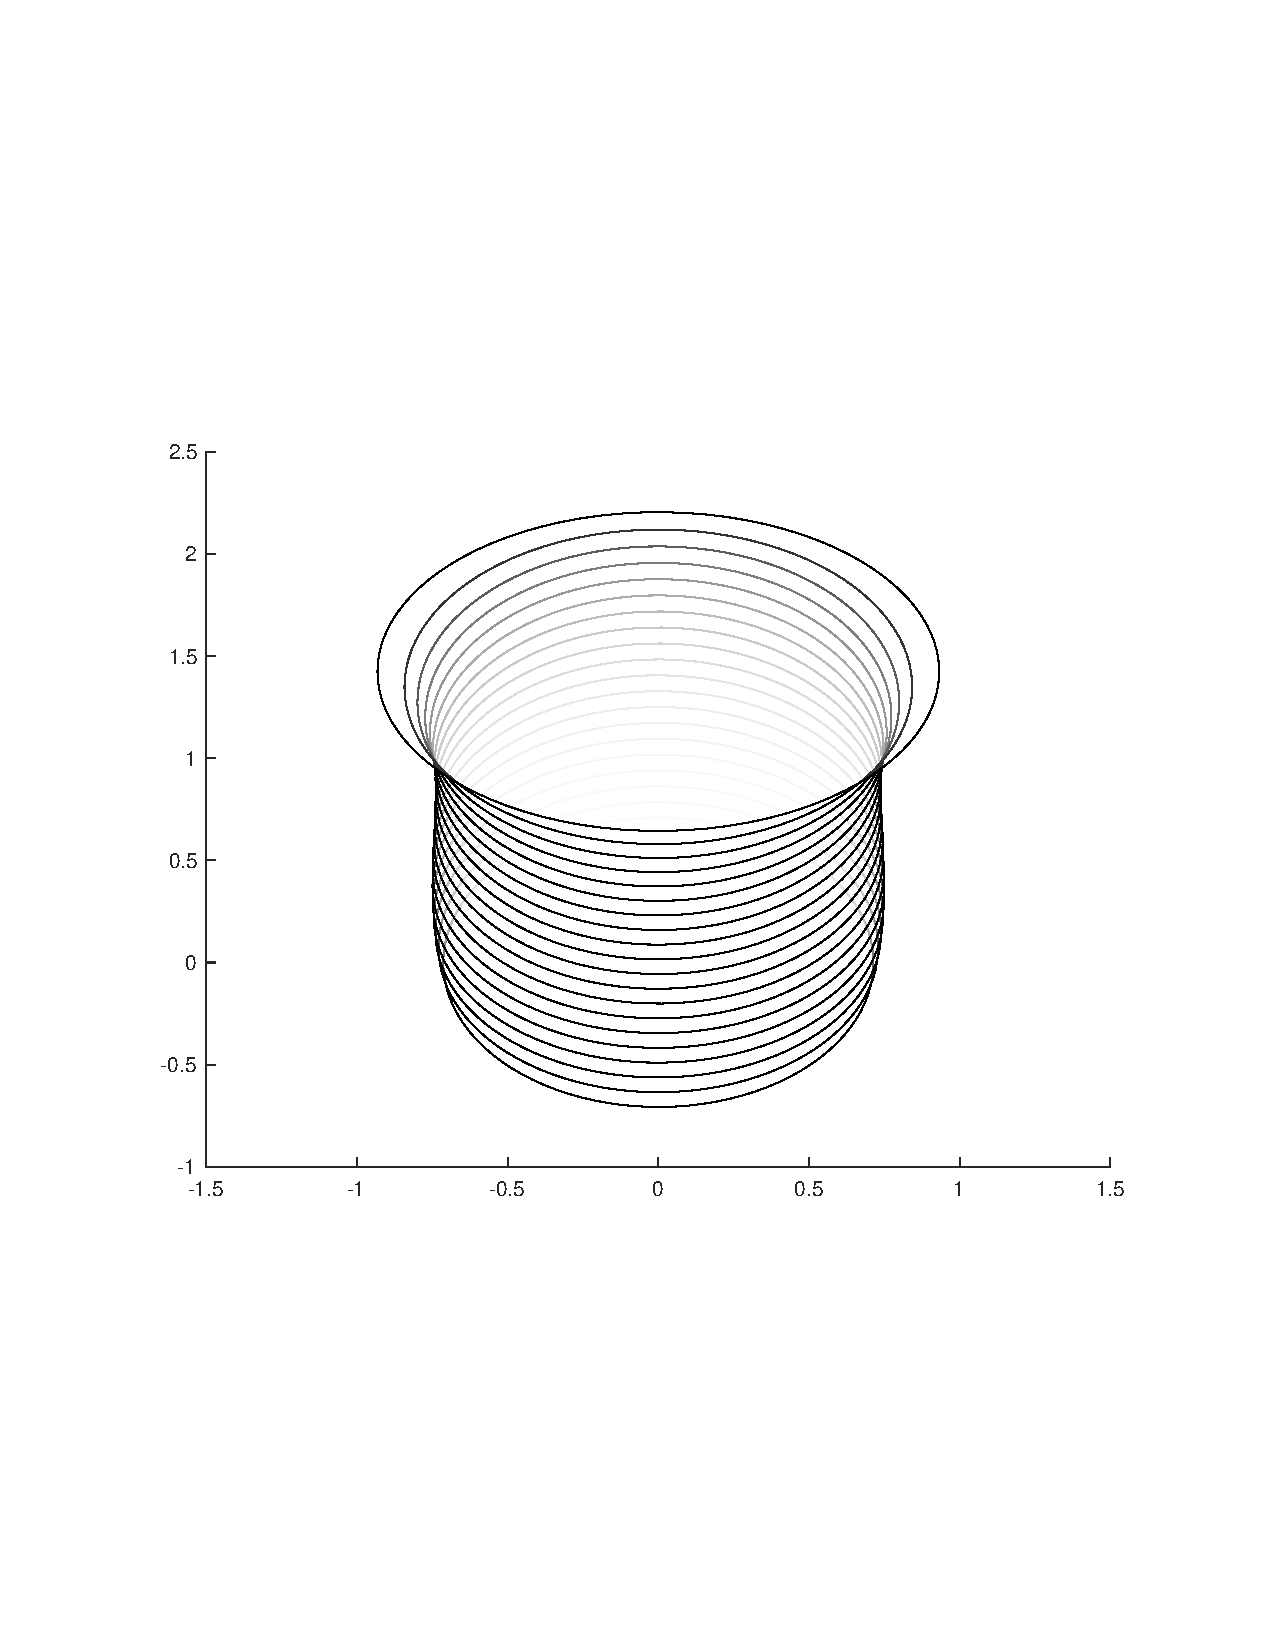
\includegraphics[width=\textwidth]{figures/experiments/unexpanded-funnel}
    \caption{The funnel around a straight trajectory for the point
      model.\newline}
  \end{subfigure}%
  \;
  \begin{subfigure}{0.5\textwidth}
    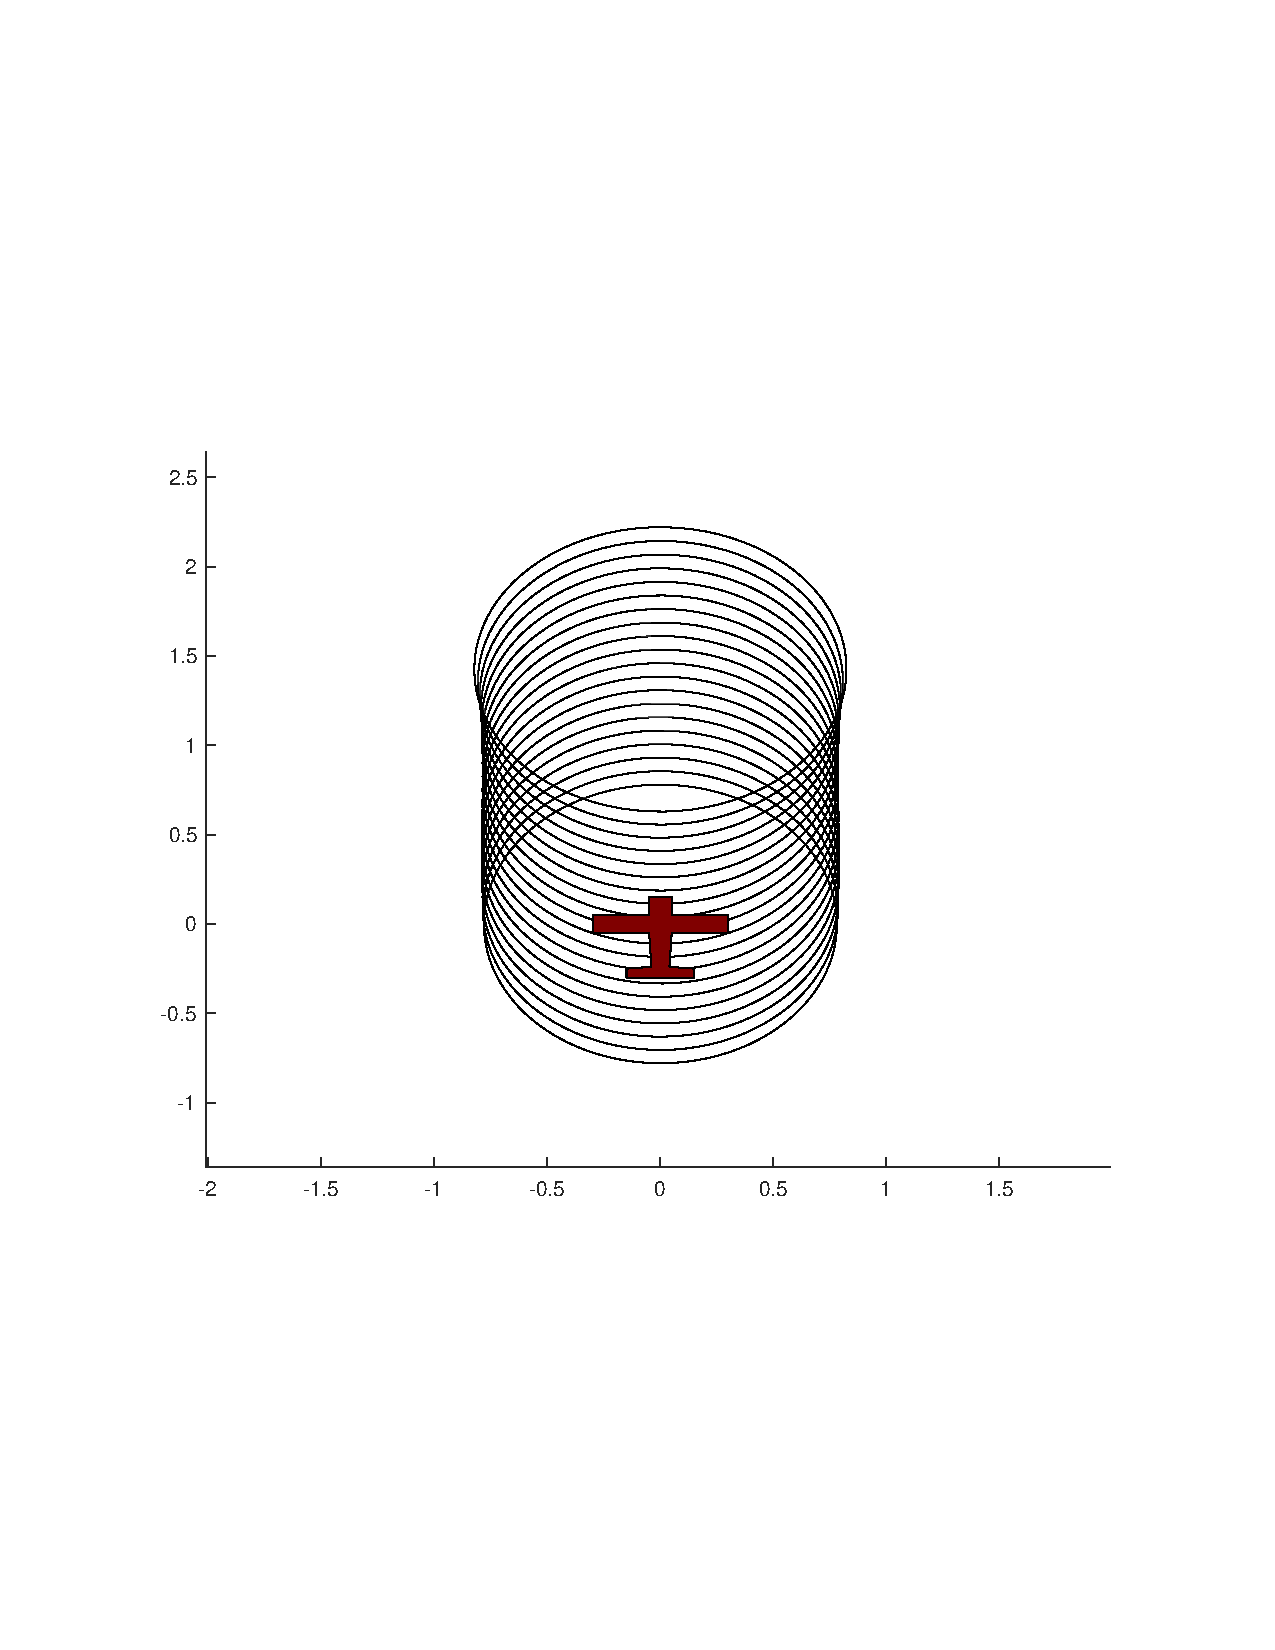
\includegraphics[width=\textwidth]{figures/experiments/expanded-funnel-with-plane}
    \caption{The funnel around a straight trajectory for the point model,
      expanded with the size of the plane.}
  \end{subfigure}
  \caption{Pictured: An unexpanded and a funnel expanded by the size of the
    simulation plane.}
  \label{fig:expanded-and-unexpanded}
\end{figure}

\subsection{The initial motion primitive set}
\label{subsec:initial-motion-primitive}

The basis set of motion primitives should be small, yet cover enough of the
finer movements of the airplane so that the motion of the airplane can be near
continuous when composed together. Thus in order to generate a `dense' set of
motion primitives \cref{alg:initial-motion-primitives-generation} is employed in
order to generate points along the arc of a circle with \(N\) different radii as
the initial points for the trajectory generator described in
\cref{subsec:generating-the-trajectories}.

\begin{algorithm}
  \caption{Generating the initial motion primitives}
  \label{alg:initial-motion-primitives-generation}
  \DontPrintSemicolon \SetAlgoNoLine

  \KwIn{%
    \(n\) - Number of points along the arch \\
    \(r_{0}\) - Initial radius \\
    \(r_{f}\) - Final radius \\
    \(s\) - Step-size (\(r_{n+1} = r_{n} + s\)) } \KwOut{\(\mathbf{X}\) -
    Endpoints matrix for the trajectory generator}

  \(\theta_{0} = \pi\) \;

  \For{\(r_{k+1} = r_{k} + s\)}{ \(\theta_{j} = \frac{\theta{0}}{2r}\) \;
    \(\theta_{stepsize} = \frac{\theta{j}}{(n-1)/2}\) \; \(\mathbf{X} \leftarrow
    (r_{k+1}, \theta=0)\) \; \For{\(i = 1 \) \KwTo \(\frac{n-1}{2}\)}{
      \(\theta_{ki} = i*\theta_{stepsize}\) \; \(\mathbf{X} \leftarrow (r, \pm
      \theta_{ki})\) \; }\; }\;
\end{algorithm}

The initial trajectories employed in the experiments can be seen in
\cref{fig:intial-trajectories-exp}, and the projected funnels overlaid a sample
in \cref{fig:sample-funnel-overlay}.

\begin{figure}
  \centering 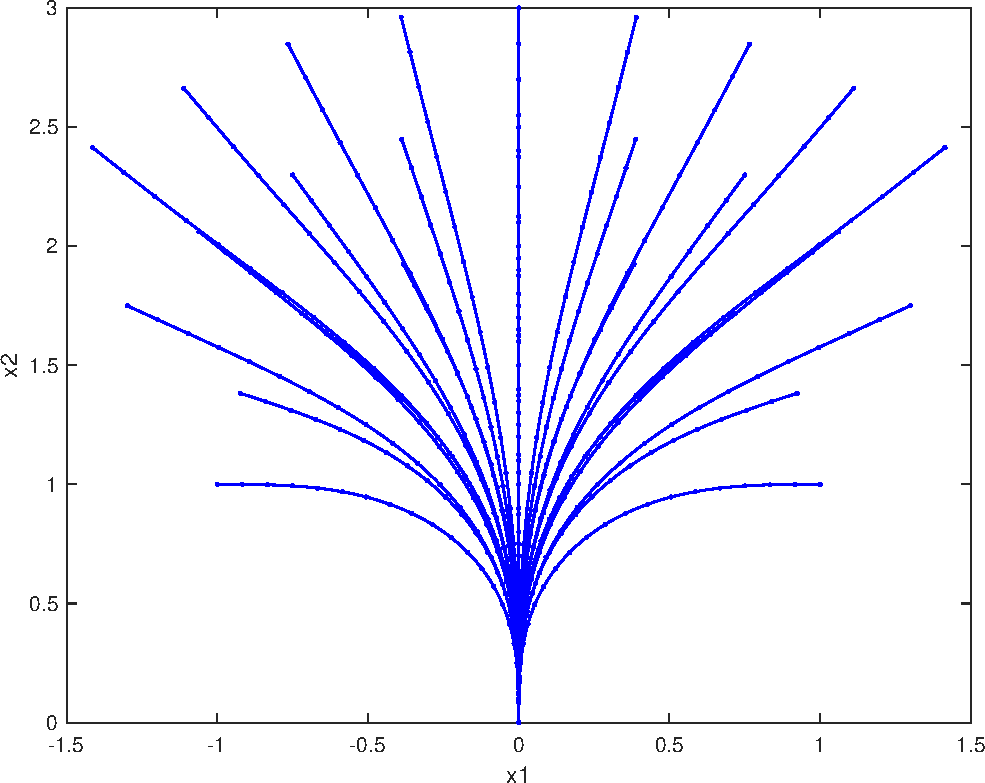
\includegraphics[scale=.7]{figures/experiments/initial-trajectories}
  \caption{The initial trajectories used in the \rrtfunnel{} algorithm.}
  \label{fig:intial-trajectories-exp}
\end{figure}

\begin{figure}
  \centering 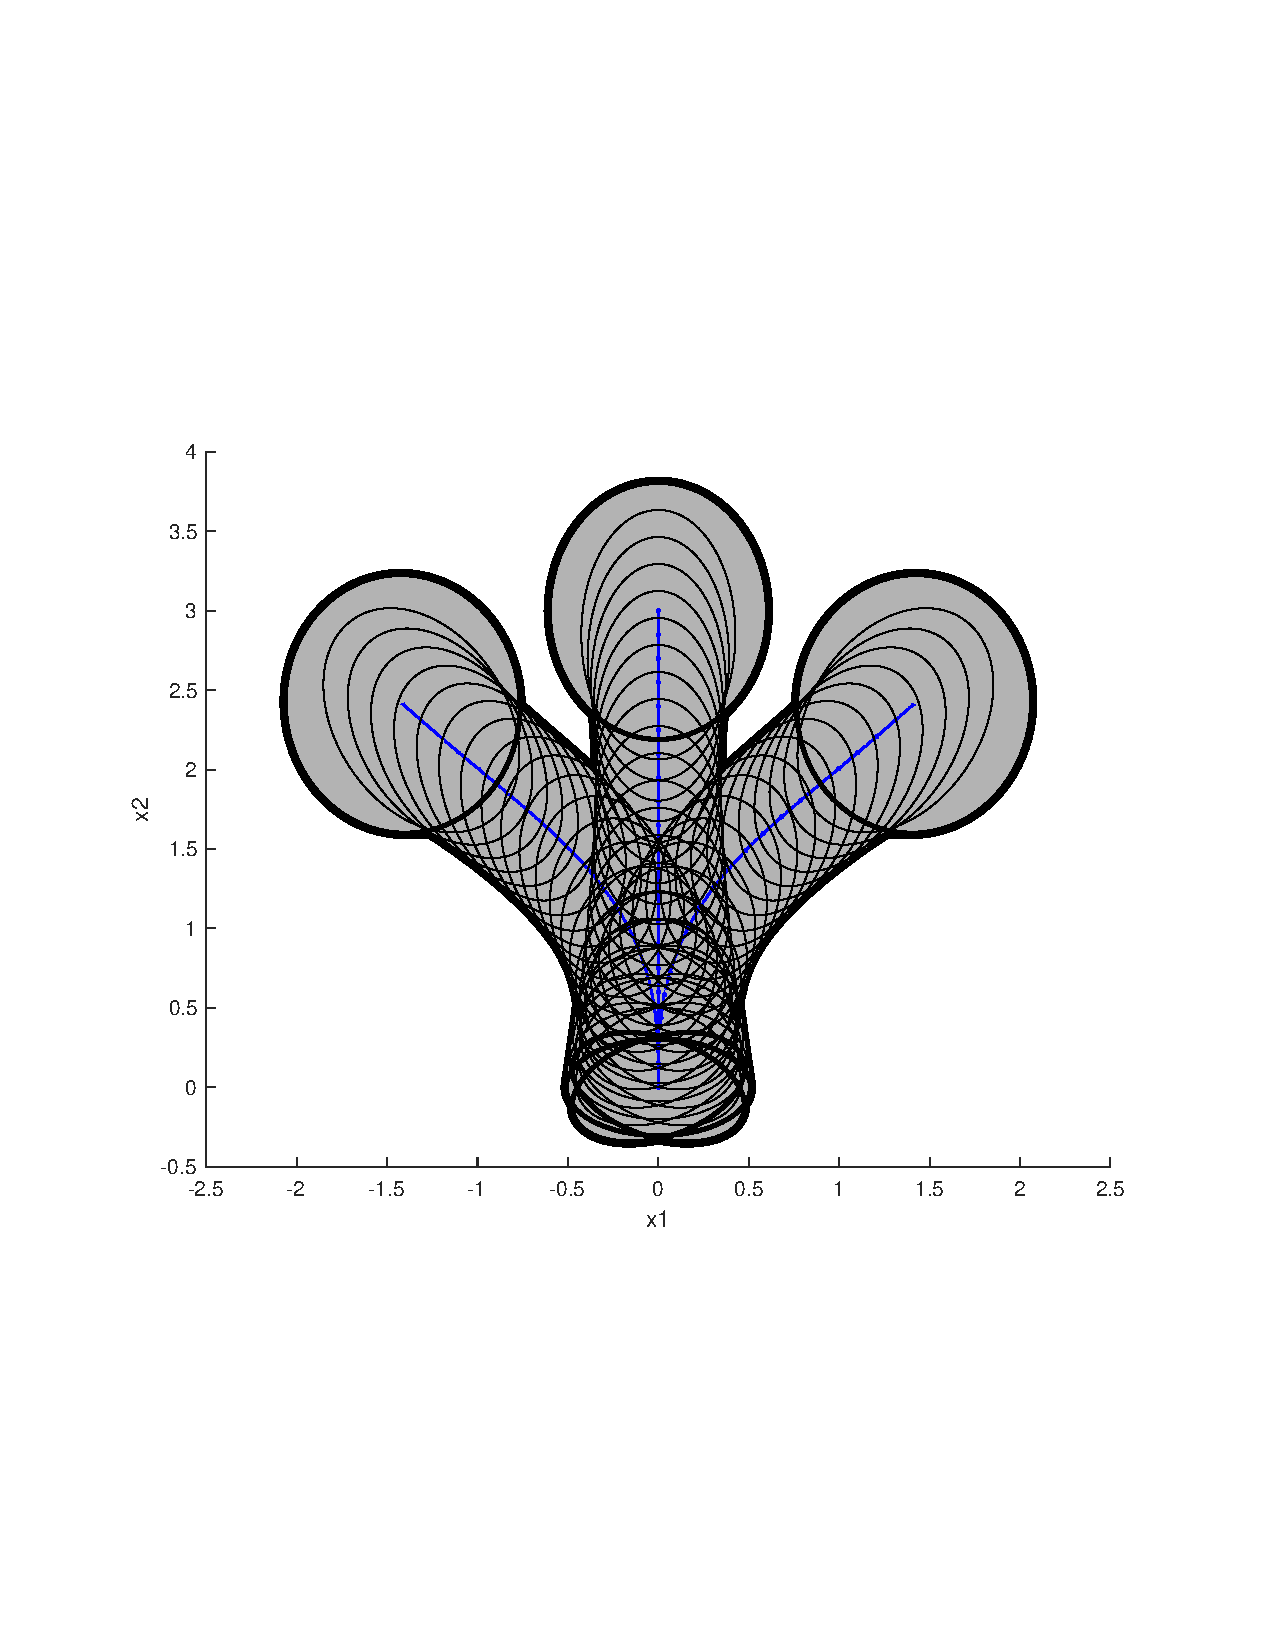
\includegraphics[scale=.7]{figures/experiments/sample-funnel-overlay} \caption{Three funnels from
    the initial trajectories with the projected funnels overlaid.}
  \label{fig:sample-funnel-overlay}
\end{figure}

\subsection{LQR cost matrices}
\label{subsec:lqr-cost}

Although the focus of this thesis is not on fine-tuning the \ac{LQR}-controller,
some amount of effort has to go into getting the cost parameters acceptable, so
that the funnels do converge. In general the strategy is penalizing the
airplane's distance from the nominal path in \((x,y,\theta)\), and be more
lenient with the energy expended by the control input. Thus path divergence is
penalized hard, and input divergence is not.

More specifically the cost matrices employed are
\begin{align*}
  R &= 0.01 \\
  Q &= \begin{bmatrix}
    40 & 0 & 0  \\
    0 & 40 & 0  \\
    0 & 0 & 4   \\
  \end{bmatrix}
  \\
  Q_{f} &=
          \begin{bmatrix}
            1 & 0 & 0   \\
            0 & 1.5 & 0  \\
            0 & 0 & 1   \\
          \end{bmatrix}
\end{align*}
where the control input is only penalized \(\frac{1}{10}\)th of the other
variables.

\subsection{Making sure that the airplane stays within the funnels during
  execution}
\label{subsec:check-vehicle-in-funnel}

\begin{figure}
  \centering 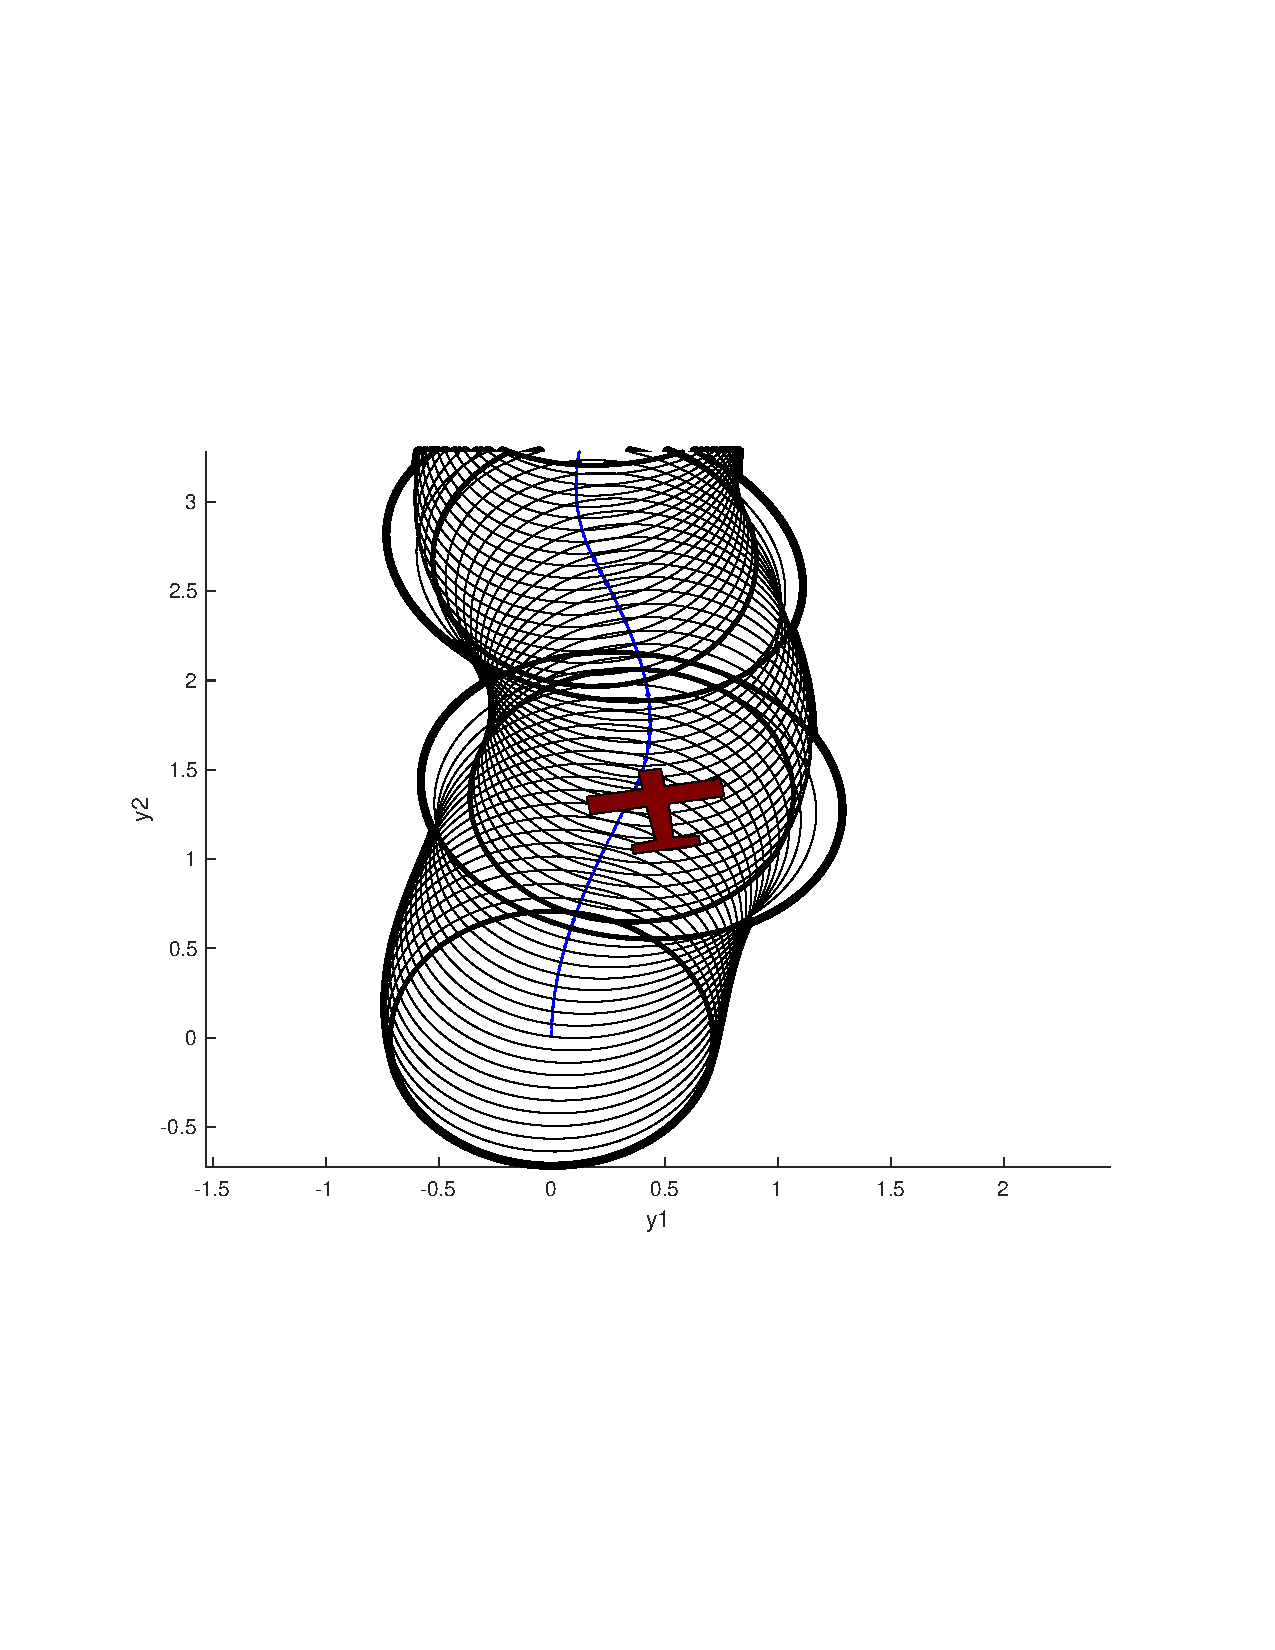
\includegraphics[width=.8\textwidth]{figures/experiments/airplane-in-funnel} \caption{A figure of the
    airplane in the funnel projected down on the xy-plane during a simulation
    run.}
\end{figure}

During the execution of the \rrtfunnel{} algorithm the planner keeps track of
the whether or not the model has left the funnel during execution, and aborts
the simulation with the emergency maneuver if the airplane happens to leave one
of the funnels at runtime. This happens if the value of the Lyapunov function is
larger than one. This will be counted in the experiments as a collision on the
part of the \rrtfunnel{} algorithm. A plot of the Lyapunov values for a
simulation run can be seen in \cref{fig:lyapunov-values}.

\begin{figure}
  \centering
  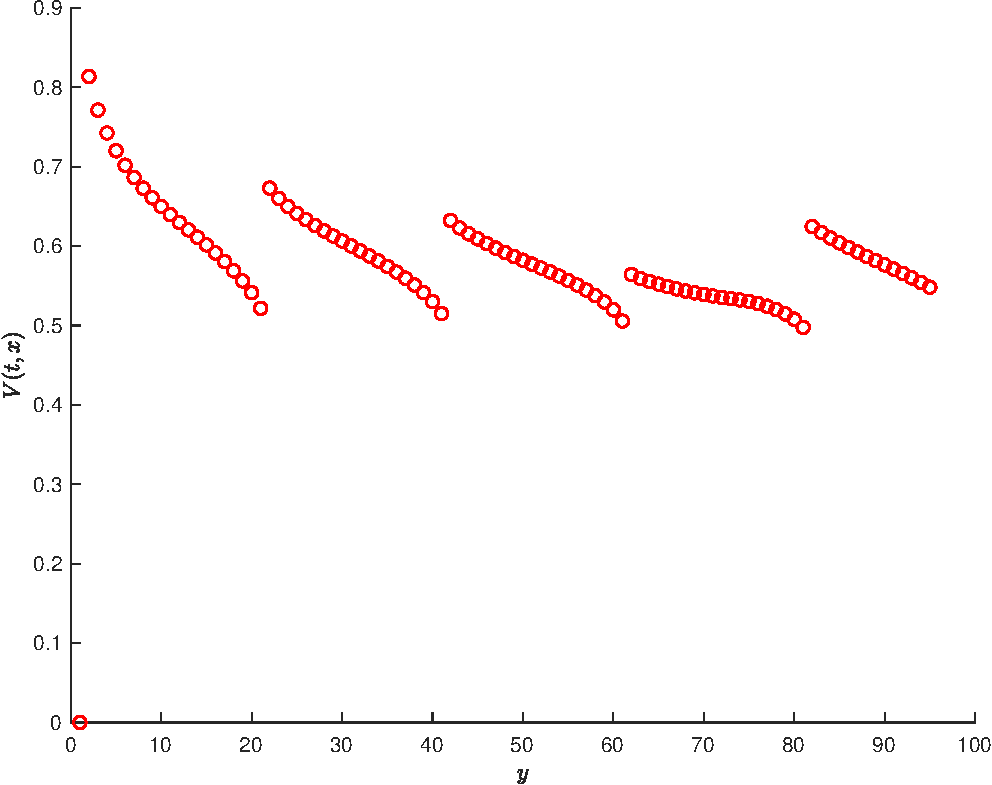
\includegraphics[width=.8\textwidth]{figures/experiments/lyapunov-values-simulation-run}
  \caption{The plot of the Lyapunov values for a simulation run at the sampling
    times \(t_k\).}
  \label{fig:lyapunov-values}
\end{figure}

\subsection{Show the funnel inlets and outlets from the funnel computations}
\label{subsec:funnel-no-composable}

Unfortunately, the funnels do not compose, and the composition testing of the
algorithm has to be left out. This is because the controller has no influence on
the speed of the airplane, and hence there is no way to make the system converge
in the direction of speed as exemplified in the~\cref{fig:funnel-conv}. The
inlet overlaid the outlets for the projected xy-funnel, and y-theta-funnel can
be found in \cref{fig:funnel-inlet-outlet} and shows this.

\begin{figure}
  \centering
  \begin{subfigure}[b]{0.4\textwidth}
    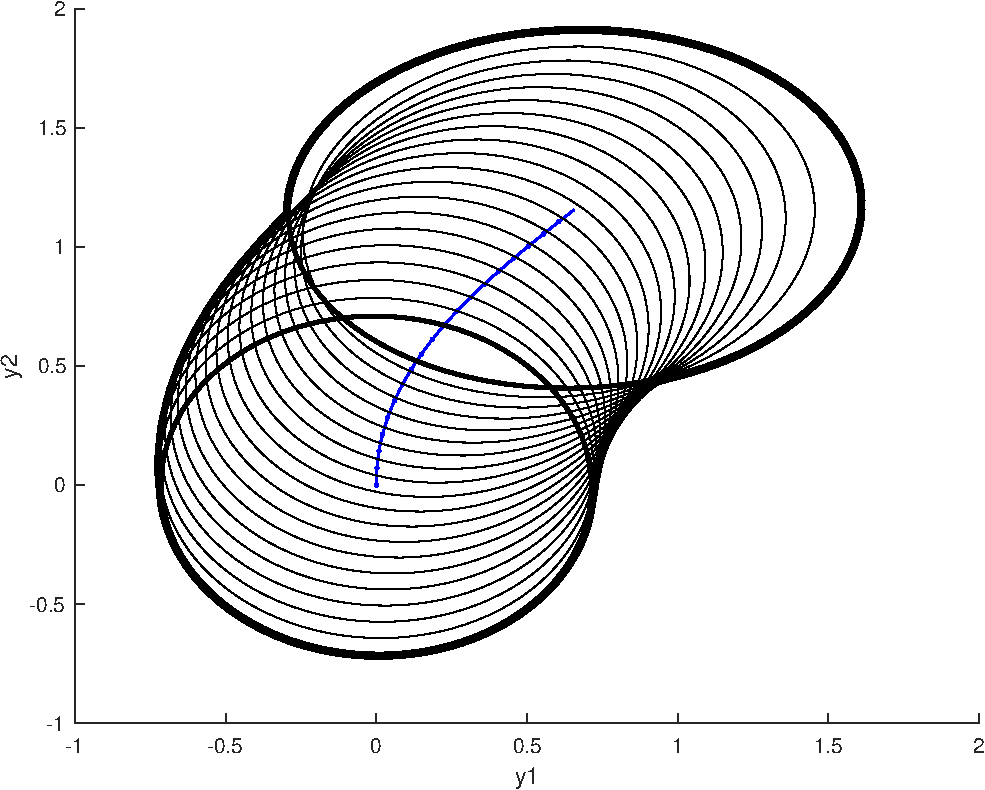
\includegraphics[width=\textwidth]{figures/experiments/sos-calculation}
  \end{subfigure}
  \quad
  \begin{subfigure}[b]{0.4\textwidth}
    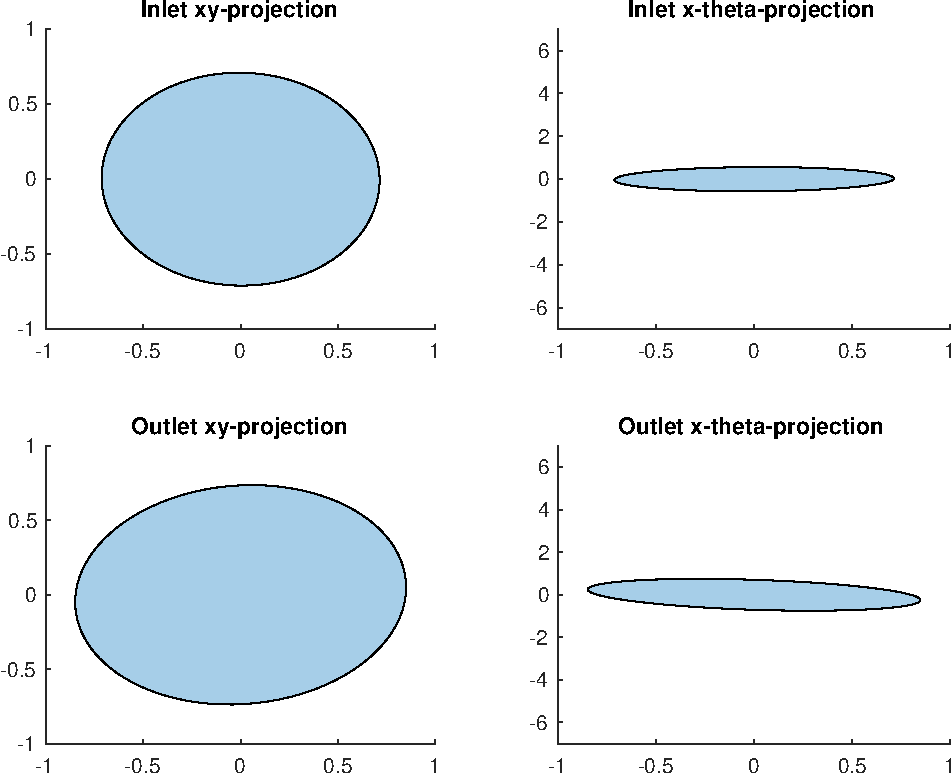
\includegraphics[width=\textwidth]{figures/experiments/sos-calculation-inlet-outlet}
  \end{subfigure}
  \caption{Pictures: A slice of the inlet and the outlet ellipsis in the x-y and
    x-theta dimensions.}
  \label{fig:funnel-conv}
\end{figure}

\begin{figure}
\centering
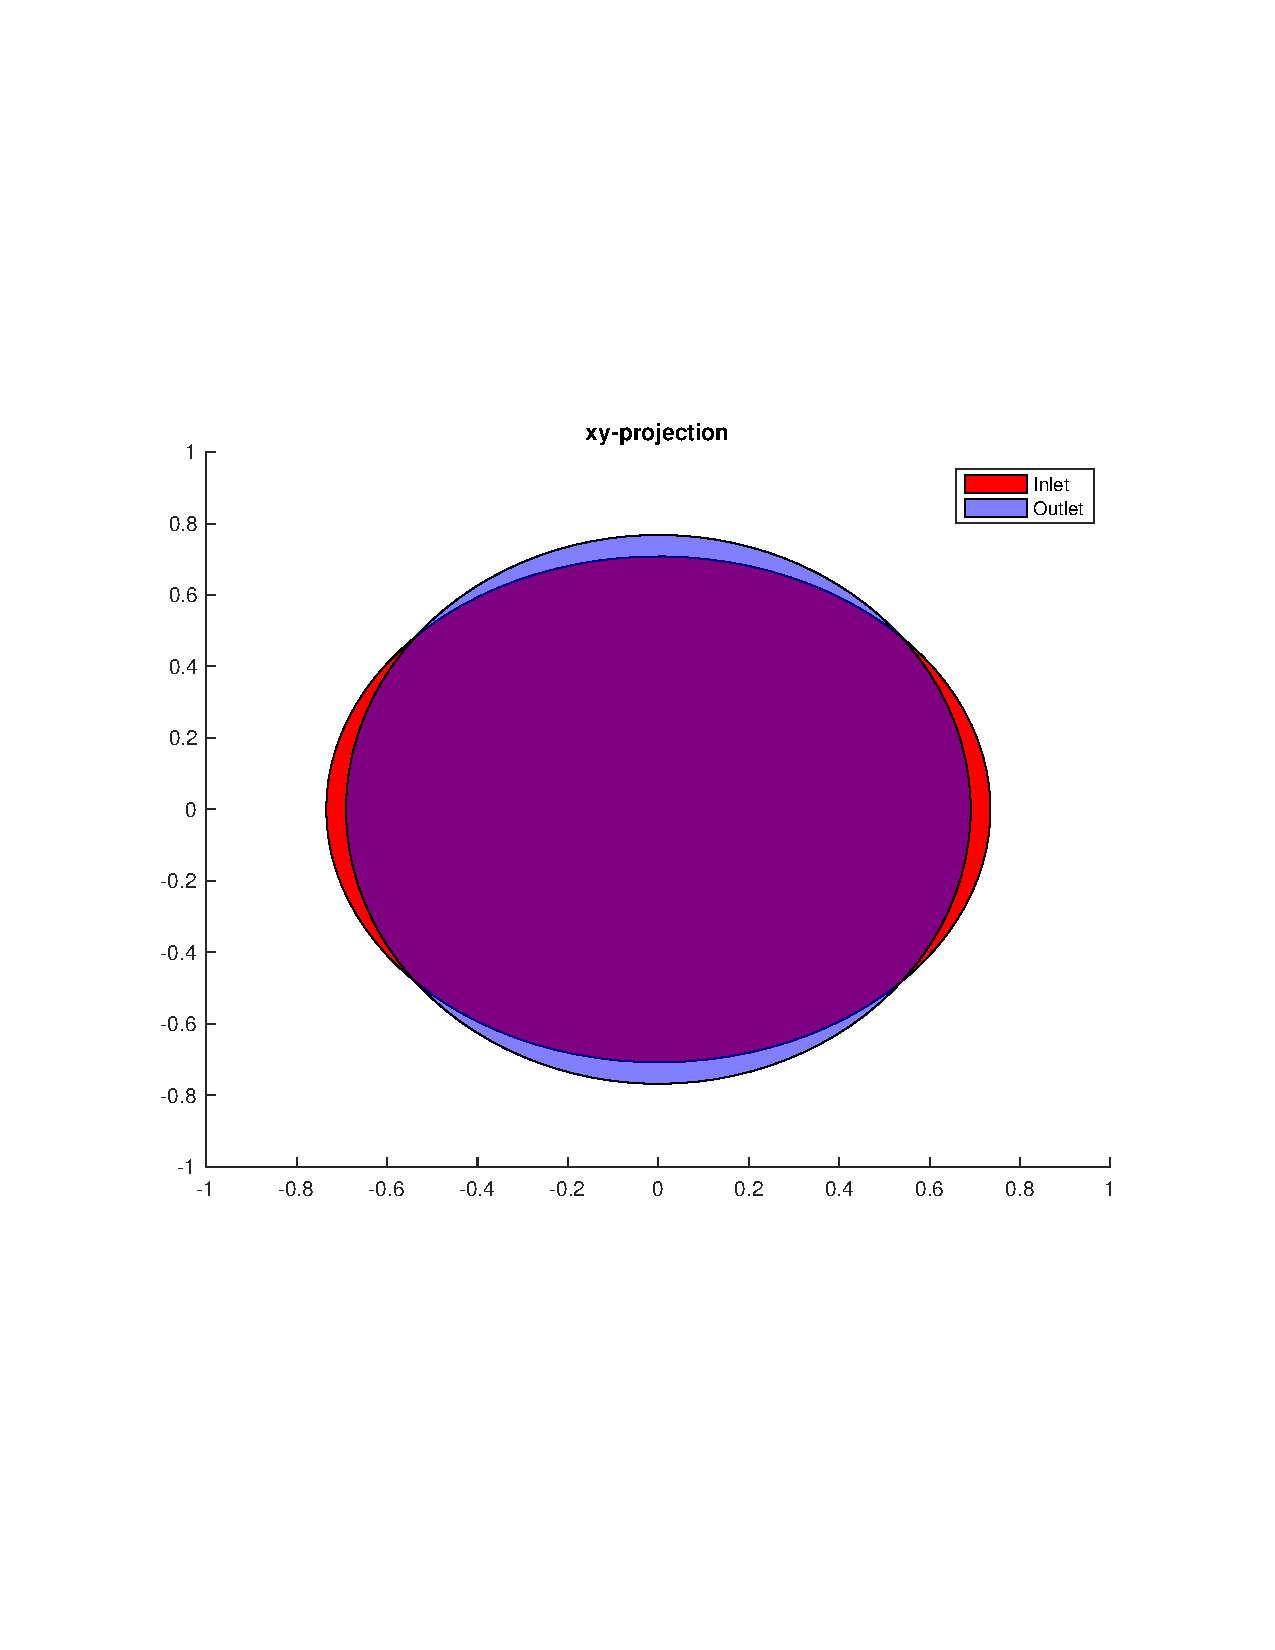
\includegraphics[width=.8\textwidth]{figures/experiments/funnel-inlet-outlet}
\caption{The projection of the funnel inlet and outlet in the xy-plane. It is
  seen that the controller is able to make the funnel converge in the
  x-direction as expected, however, it has no control in the y-direction, as
  there is no controller steering the speed of the vehicle.}
\label{fig:funnel-inlet-outlet}
\end{figure}

\section{Results}
\label{sec:experiments-final}

The experiments will run the \rrtfunnel{} against a benchmark regular RRT
planner with the motion primitive set pictured
in~\cref{fig:intial-trajectories-exp} on the forest traversal problem pictured
in~\cref{fig:simulated-forest}.

The benchmark-planner is an \ac{RRT} algorithm using the same motion primitive
set as the \rrtfunnel{} algorithm, with the same \ac{LQR} controller, and the
same distance metric. The difference is that it does not take uncertainty into
account, and instead maximizes the distance to the nearest obstacle as the
extension operator \ie{}
\begin{equation}
  \max_{i}\min_{t,j}(\vect{x}_{i}(t), o_{j})
\end{equation}
where \(x_{i}(t) \in \mathcal{T}\), is a trajectory from the basic motion
primitive set, and \(o_{j} \in \modelobstacle{}\) is an obstacle in the
configuration space \(\modelconfigurationspace{}\).

The end goal is set so that it will not take pose into account, and will only be
concerned with getting within an \(\epsilon\) of the \((x,y)\) in the test map.
For all the experiments below, an \(\epsilon\) of 5\si{\metre} is given to the
planners.

Each test-run will be run in a forest generated with the \textit{Poisson
  process} method from~\nameref{sec:Poisson-Process}, and an intensity parameter
(\(\lambda = 0.1,0.2,0.3\)) respectively, which should yield a pretty dense
forest, and hence make collisions more likely to happen.

The experiments will record the number of collisions for each algorithm across
all test-runs. The planners will run in the same environment for each test, with
the same initial starting point, but the environments will be different for each
run, as the Poisson process generating the obstacle forest is random in nature.
With this test setup the difference between a planner which takes into account
uncertainty should become evident.

Before the experiments are run, all individual funnels in the base set are run
with a hundred simulations runs from random starting positions in its inlet, to
check if the invariant holds, and that the airplane stays within the funnel at
all times. 

Uncertainty is added in terms of additive noise with \(w = -0.3\)\si{m.s^{-1}}
in the world x-direction. Below are the results from a hundred test-runs with
the test setup from above:

\begin{figure}
  \centering 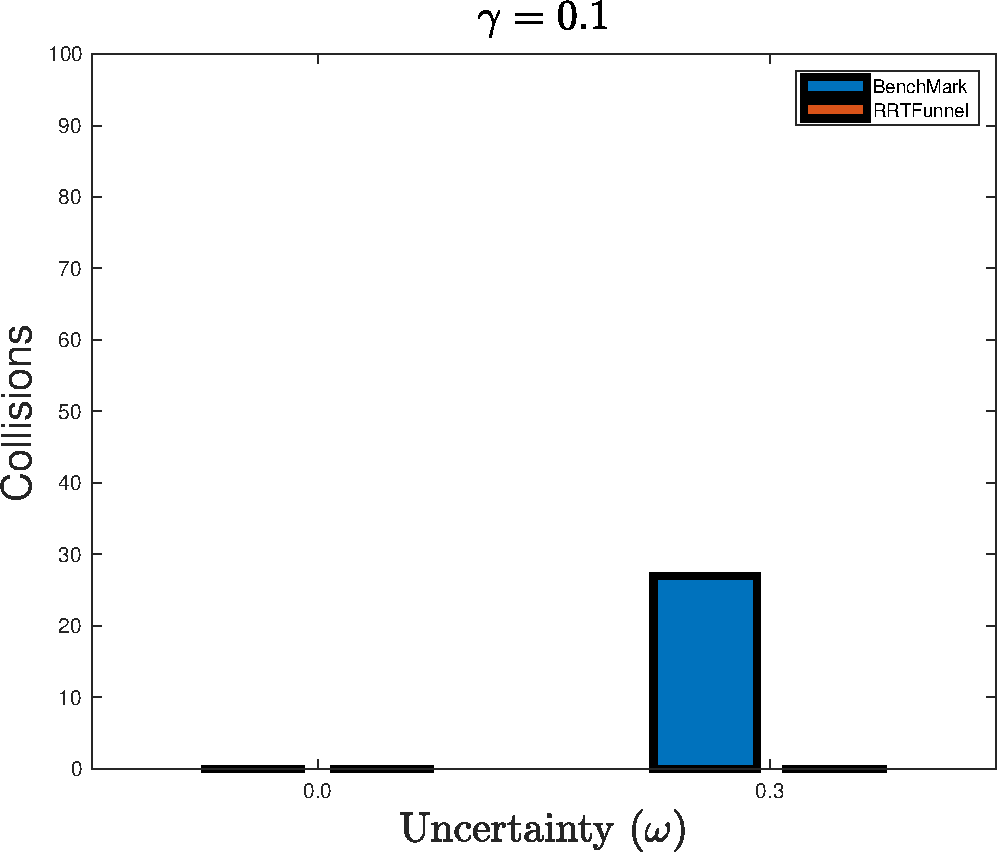
\includegraphics[width=\textwidth]{figures/experiments/ResultPlot01}
  \caption{Results for forest density = 0.1}
  \label{fig:result0.1}
\end{figure}

\begin{figure}
  \centering \fbox{%
    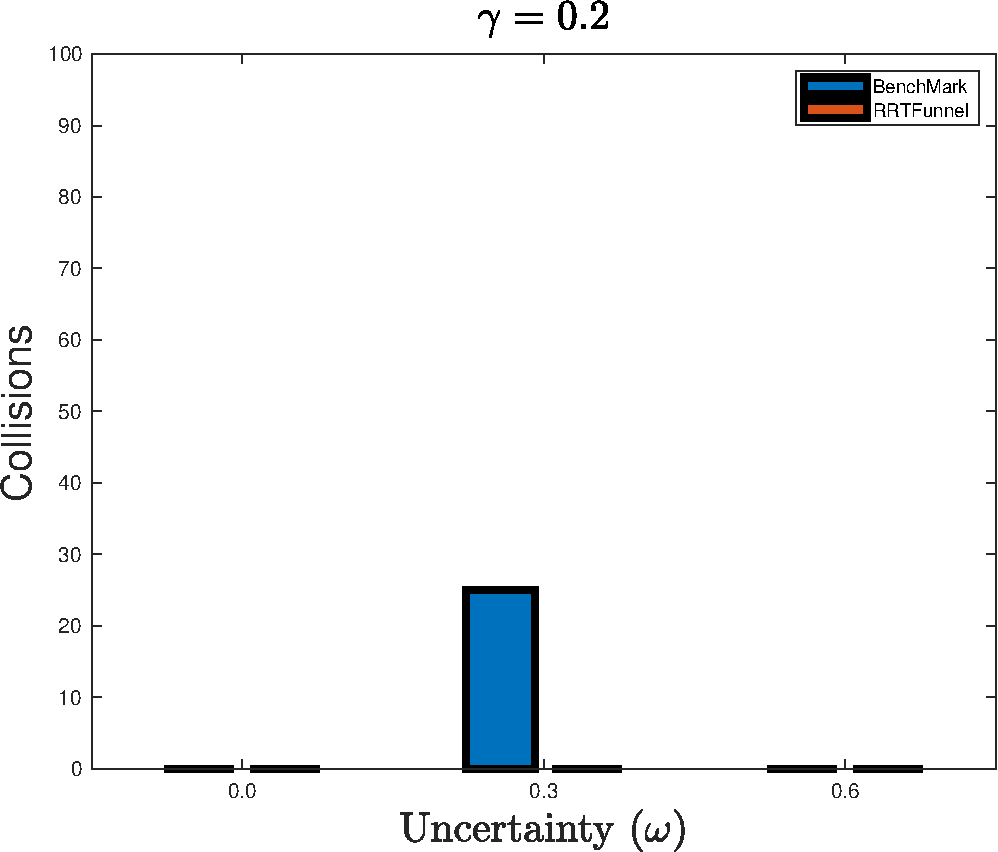
\includegraphics[width=\textwidth]{figures/experiments/ResultPlot02}}
  \caption{Results for forest density = 0.2}
  \label{fig:result0.2}
\end{figure}

\begin{table}
  \begin{tabular}{ll*{6}{d{2.2}}}
    \toprule
    {}&{}& \multicolumn{3}{c}{Benchmark} & \multicolumn{3}{c}{\rrtfunnel{}} \\ \cmidrule(r){3-5} \cmidrule(l){6-8}
    {}&{}& \mc{\(w=0\)} & \mc{\(w=3\)} & \mc{\(w=6\)} & \mc{\(w=0\)} & \mc{\(w=3\)} & \mc{\(w=6\)} \\
    \cmidrule{3-8}
    \multicolumn{2}{l}{Density} \\ \cmidrule{1-2}
    {}& \(\lambda=0.1\)   &      0 &        27 &      0 &       0 &           0 &        0 \\
    % {}& median &      34.39 &        29.30 &      \textbf{23}.\textbf{09} &       35.79 &           29.49 &        25.88 \\
    {}& \(\lambda=0.2\)    &      0 &        32 &      0 &       0 &           0 &        0 \\
    {}& \(\lambda=0.3\)   &      0 &        38 &      0 &       0 &           0 &        0 \\
    % {}& R5.0   &      \textbf{77}.\textbf{26} &        85.77 &      80.63 &       77.19 &           83.93 &        80.74 \\
    % {}& R10.0  &      71.23 &        73.80 &      \textbf{68}.\textbf{16} &       71.80 &           72.81 &        69.69 \\
    \bottomrule
  \end{tabular}
\end{table}

\begin{figure}
  \centering 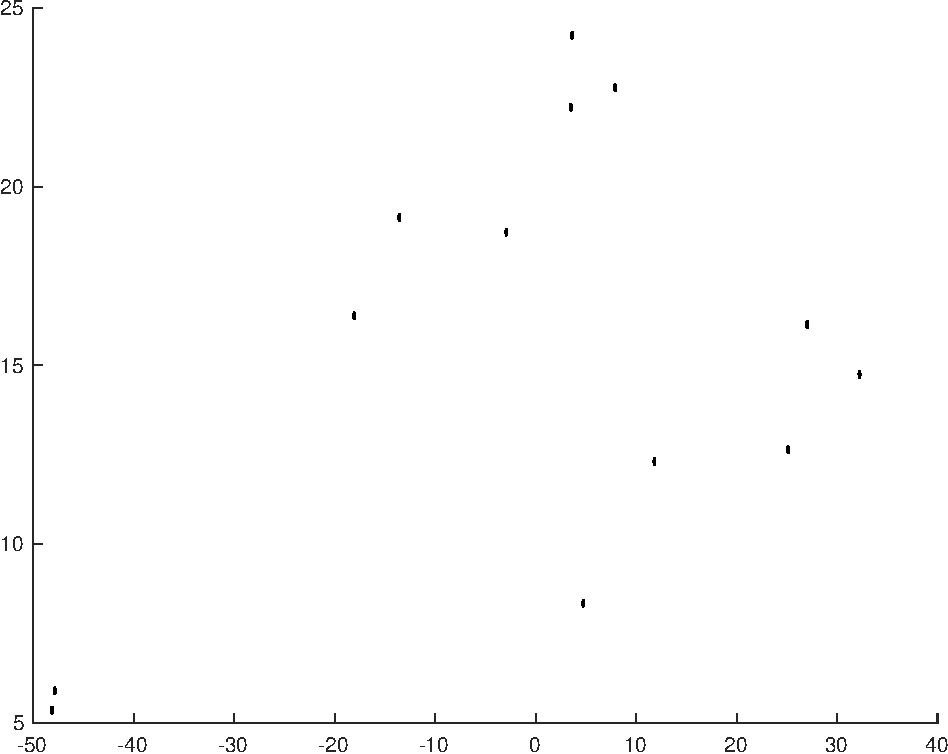
\includegraphics[width=.8\textwidth]{figures/experiments/FunnelGraphExperiment}
  \caption{Pictured: One solution for the \rrtfunnel{} algorithm for the
    experiment setup.}
\end{figure}